\chapter{学位论文写作细则}
\label{cha:fourthsection}

学位论文很多的错误源于凌乱的格式。

为规范学位论文写作,本章结合工科学位论文的特点,参照学术出版规范,就图、表制作,名词、术语、单位、符号、数量等的使用规范化进行了说明。

\textcolor{red}{(论文中所有图表清晰,字体、格式一致,图标题在图下方,表标题在表上方。图表引用和图表不跨页,确有需要跨页不超过1页)}


\section{关于图}
\label{sec:parameters}
参照CY/T 170-2019《学术出版规范 插图》标准执行。

论文中的图一般居中放置,大小要合适,宽度不得超过文字边缘,图中文字一般不大于五号;图像分辨率应尽量不低于300 dpi;若为自画图,尽量采用中文标识,图中文字经缩放后,字号不得大于五号;图注也只需加注中文,宋体,五号。若引用文献中的图,应在图注最后标注引用,图注后无需加标点符号。文中所有的图都应予编号,图序号按“章”进行编号,如图\ref{Fig4-1}所示:
\begin{figure}[!htbp]
    \centering
    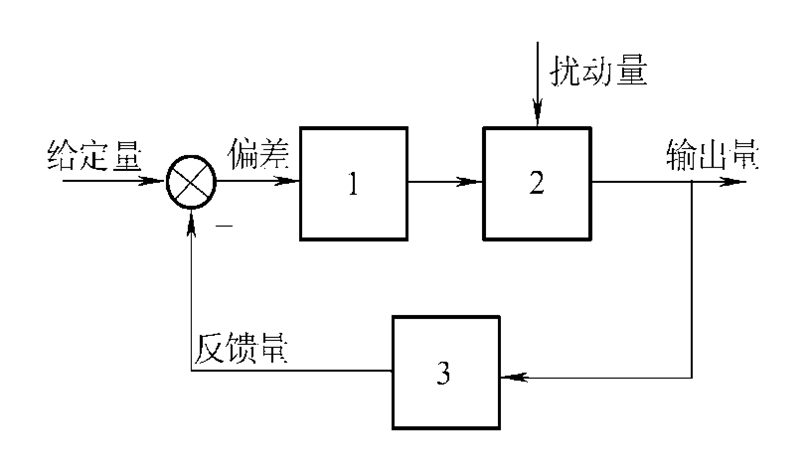
\includegraphics{figures/Fig4-1.png}
    \caption{闭环系统示意图}\label{Fig4-1}
\end{figure}
制作图时请注意:
\begin{enumerate}
    \item[(1)] 内容与形式应力求统一。风格、体例应一致。线条图应清晰,线型选用、线条粗细应规范,色调准确,图形布局合理、大小适当。连续色调图应清晰,层次感和饱和度适当。
    \item[(2)] 每幅都得有图题。图题应准确、简明地阐释该图内容。
    \item[(3)] 图应与正文内容相关。应选择能有效传达关键信息的图,应具有自明性、简明性、科学性和艺术性。
    \item[(4)] 结构示意图、原理示意图和流程图的设计制作应符合现行的国家标准或行业标准。
    \item[(5)] 坐标曲线图的坐标轴、标值线的画法应规范,标目、标值、坐标原点应标注完整、规范、统一。
    \item[(6)] 图中涉及标志用图形符号、设备用图形符号和技术文件用图形符号应符合现行的国家标准。图中的术语、数值、符号等应与正文其它图中的表述一致。
    \item[(7)] 图应尽量与相应的文字靠近,根据排版可放在文字的下方或上方。各章节不能因为图的原因出现大段留白的现象。
    \item[(8)] 图中应有对于需特别说明问题部分的标识说明,如图像中需给出比例尺,在彩图中给出Color bar等。说明字体与比例尺的字体应至少比正文小一号。
\end{enumerate}





\section{关于表格}
\label{sec:results}
学位论文中的表格要使用三线格,居中放置。表格题目应居中放置于表格顶端。仅需提供中文表头,表头及表中文字应小于正文字号,一般为宋体,五号;若其中含英文或数字时,字体为Times New Roman,五号。表格题目与表格尽量不要分页。实在需要分页时,请在下一页续表。若该表完全源于文献,应在表格题目最后标注引用。标头最后不加标点。如表\ref{Tab4-1}所示:

\begin{table}[htbp]
  \centering
  \caption{表格示例}
    \begin{tabular}{ccccc}
    \toprule
    Aaa & Bbb & Ccc & Ddd & Eee \\
    \midrule
    1-1  & 1-2  & 1-3 & 1-4 & 1-5 \\
    2-1  & 2-2  & 2-3 & 2-4 & 2-5 \\
    3-1  & 3-2  & 3-3 & 3-4 & 3-5 \\
    4-1  & 4-2  & 4-3 & 4-4 & 4-5 \\
    \bottomrule
    \end{tabular}%
  \label{Tab4-1}%
\end{table}%

一般情况下,表应放在文字的下面,有时依据排版的需要,也可以放在文字上方。但无论如何,图应尽量与文字靠近。

\begin{enumerate}
    \item[(1)] 表格序号按“章”进行编号,如第3章第1个表为“表3-1”,以此类推。
    \item[(2)] 表格内容与正文配合应相得益彰,内容适合用表表达。
    \item[(3)] 表格应具有自明性和简明性,栏目设置应科学。
    \item[(4)] 表格中的数据应具有完整性和准确性。
    \item[(5)] 表格中连续数的分组应科学,不得重叠和遗漏。
    \item[(6)] 表格中的数值修约和极原数值的书写应符合GB/T 8170的规定。
    \item[(7)] 表格中的量和单位的名称、符号及书写应符合国家标准GB3100~3102—93量和单位的系列标准和相关行业标准。
    \item[(8)] 表格中数字形式的使用应符合GB/T 15835规定。
    \item[(9)] 表格中的科学技术名词应符合CVT 119的规定。
    \item[(10)] 表格中的术语、数值、符号等应与正文以及同一文本中其他表格中的表述一致。
    \item[(11)] 全书的表格的表号、表题,表头、表身、表注的格式应统一。
\end{enumerate}

\section{名词、术语}

学位论文存在大量的专业名词与专业术语,针对同一内容的名字、术语有多种表达方式时,原则上以关系最为密切的学科为准,并尽量符合最新的国家或行业规程、规范。若属全国科学技术名词审定委员会最新公布的各类学科的“名词”,则须严格执行,且在全文中统一。

外国专有名称在释文中首次出现时,应附原文和简称。例如:“美国垦务局(United States Bureau of Reclamati,USBR)”、“美国大坝委员会(United States Committee On Large Dams,USCOLD)”。在同一条目中再次出现时可采用中文或英文缩写。


\section{符号、单位的使用}
标点符号的使用,应符合国家标准GB/T 15834—2011《标点符号用法》。
\begin{enumerate}
    \item[(1)] 论文中的计量单位应采用法定计量单位(简称法定单位),应符合国家标准GB 3100~3102—93量和单位的系列标准和相关行业标准。
    \item[(2)] 表格及插图中,使用单位符号,不使用单位名称和单位中文符号。叙述性文字中,优先使用单位符号。必要时,可使用单位名称,但不可使用单位中文符号。如:流量为11400
    \item[(3)] 两个物理量(量值加单位)在表示范围时,两个量值用波浪线“~”连接后使用一个计量单位,如:应写作800~1500 m3/s,而不写作800m3/s~1500 m3/s。
\end{enumerate}


\section{数字的使用}

数字的使用应符合国家标准GB/T15838—2011《出版物上数字用法》,同时应符合相关行业标准。

以下情况应使用阿拉伯数字:
\begin{enumerate}
    \item[(1)] 统计表中的数值,如:正负整数、小数、百分数、分数、比例。
    \item[(2)] 物理量量值,如:150 m3/s,200 kg,注意数量与单位之间应有空格。
    \item[(3)] 非物理量量值。如:21.35元,480人。
    \item[(4)] 当阿拉伯数字与汉字数字混用时,要顾及上下行文的协调一致。
    \item[(5)] 两个百分数表示范围时,要使用两个百分号,如15%~20%,不可写成15~20%。
    \item[(6)] 专业性科技出版物上的多位数字,应从小数点算起,每三位留空半个数码位置,不采用传统的以千位撇“,”分节的办法,如3800000应写成3 800 000,或写成380万,而不要写成3,800,000。
\end{enumerate}

以下情况应使用汉字数字:
\begin{enumerate}
    \item[(1)] 定型的词、词组、成语、惯用语或具有修辞色彩的词语中作为词素的数字。如:星期六、四氧化三铁、五省一市、“八五”计划、第三季度等。
    \item[(2)] 相邻两个数字并列连用表示概数,连用的两个数字间不得用顿号“、”隔开。如:二三米、十三四吨、一千七八百元。
    \item[(3)] 不是出现在具有统计意义的一组数字中的整数一至十。如:一个人、三本书、五个百分点等。
    \item[(4)] 带有“几”的数字,表示概数。如:十几天、几千年等。
\end{enumerate}

\section{其它应该注意的问题}

\subsection{关于文献引用}

在学位论文撰写中,凡是文字、图、表来自于参考文献的,必须要加注文献信息。国际惯例:与他人文章有20个字连续雷同的就是抄袭。抄袭是必须严禁的行为,否则害人害己。建议大家最好用自己的理解来撰写相关内容,特别是第一章绪论中更应注意。

在引用参考文献时,不要将文献标识直接写在某一小节的标题上,这将被视为整节内容都是引用;如有某几句话完全来自文献的,则在这部分内容的最后一句的结束加文献标注。

在课题组内部,经常出现多位同学做相近的课题,或课题的关联性较大。每个学生介绍研究背景或实验室材料与方法时,请尽可能用自己理解后的语句去撰写,以避免雷同,千万不要图省事将前一届学生的论文大段地照搬过来。有些图若是能自己画的,最好自己重新画一遍,以示区分。

\textcolor{red}{硕士学位申请人的文献阅读量一般不少于40篇,其中外文文献一般不少于1/3;近五年的论文一般不少于1/3;绪论部分应对所读文献加以分析和综合。}

参考文献格式

中文书刊:作者按中文写法,姓在前、名在后;英文书刊:作者按英文习惯写法,如名在前、姓在后,名用首字母缩写、姓用全称。一般6人以内须列出全部作者,6人以上写6人再加“等”(英文加“et al”))。每个参考文献的最后不加标点符号。

(1)图书:最多列出6个作者,作者与作者之间用逗号分隔. 书名. 版本(第×版). 译者. 出版地: 出版者, 出版年. 起页-止页(可选)

(2)期刊:最多列出6个作者,作者与作者之间用逗号分隔. 文章名. 期刊名(全称). 年号, 卷号(期号): 起页-止页或论文编号

(3)会议论文集:最多列出6个作者,作者之间用逗号分隔. 文章名. 见(英文用“in”):会议名称(或论文集). 会议城市, 国家, 会议时间, 出版者, 出版年: 起页-止页

(4)专利:专利申请者. 专利题名. 专利国别, 专利文献种类, 专利号, 出版年

(5)学位论文:作者. 题名:[博士(或硕士)学位论文]. 保存地点: 保存单位(如华中科技大学, 年份)

参考文献(举例)
\begin{enumerate}
\renewcommand{\labelenumi}{[\theenumi]}
\item	闫明礼, 张东刚. CFG桩复合地基技术及工程实践(第二版). 北京: 中国水利水电出版社, 2006

\item	M. Chalfie, S. R. Kain. Green fluorescent protein: properties, applications, and protocols. Hoboken, New Jersey: Wiley-interscience, 1998

\item	詹向红, 李德新. 中医药防治阿尔茨海默病实验研究述要. 中华中医药学刊, 2004, 22(11): 2094-2096

\item	E. S. Lein, M. J. Hawrylycz, N. Ao, M. Ayres, A. Bensinger, A. Bernard, et al. Genome-wide atlas of gene expression in the adult mouse brain. Nature, 2007, 445(7124): 168-176

\item	M. L. Bouxsein, S. K. Boyd, B. A. Christiansen, R. E. Guldberg, K. J. Jepsen, R. Müller. Guidelines for assessment of bone microstructure in rodents using micro–computed tomography. Journal of Bone and Mineral Research, 2010, 25(7): 1468-1486

\item	Y. Shunsuke, A. Masahide, K. Masayuki, M. Yoshizawa. Performance evaluation of phase-only correlation functions from the viewpoint of correlation Filters, in: 2018 Asia-Pacific Signal and Information Processing Association Annual Summit and Conference (APSIPA ASC), Honolulu, HI, USA, 12-15 Nov. 2018, Proceedings of the IEEE, 2019: 1361-1364

\item	T. Yao, J. Wan, P. Huang, X. He, F. Wu, C. Xie. Building efficient key-value stores via a lightweight compaction tree. ACM Transactions on Storage, 2017, 13(4): 1-28

\item	刘加林. 多功能一次性压舌板: 中国, ZL92214985. 2 [P]. 1993

\item	李清泉. 基于混合数据结构的三维GIS数据模型与空间分析研究[博士学位论文]. 武汉: 武汉测绘科技大学, 1998

\end{enumerate}

注释体例的基本内容、结构与位置

(1)基本内容与结构

“注释体例”含“资料性注释”和“内容性注释”两方面,合一编排。

(2)位置

正文内需注释之处依次排注号,释文于当页下部逐条依次编排。可在正文和页下注之间划一道分隔线,或通过不同的字体将二者区分开来。

(3)排版

【字体】中文:小五,宋体;英文:times new roman 9号字体;

【行距】单倍行距;

【段落】顶格写,无首行缩进,也无左缩进;

【序号】用①这种格式,序号后空一个字符,每页重新编序;

【页码】中文:第х-х页,如 第16-17页。英文:pp.х~х,如pp.5~8, 单页用pх,如p19.

【标点符号】中文使用中文状态下标点符号,英文使用英文状态下标点符号,切忌混用。

\textcolor{red}{以下是几个例子, 注意, 中文参考文献需要额外增加一个 lang="chinese"}
~\\
期刊论文举例:

Pan等人提出了一种全新的算法\cite{pan2018classification, pan2014cell, song2013asynchronous, lin2022adaptive}。

~\\
会议论文举例:

XXXXxx\cite{li2021large}

~\\
图书举例:

xxxxxx\cite{shavlik1990readings, yan2006CFG}

~\\
学位论文举例:

xxxxxx\cite{jxd1996, CCPT}




\subsection{公式}
公式中主要字母的字号与正文一样(即小四号),尽量避免图片转贴过来的公式。公式编号根据章节按顺序进行编排,如第2章第3个公式,标注为2-3,将公式编号以右对齐方式排列,但注意公式是以居中的格式排列的(类似教材中的通用格式)。

\subsection{本章小结}
本章主要介绍学位论文写作的规范化要求,包括图、表制作及其与正文的对应关系;专业名词、术语、单位、符号及数字的使用等。




